\noindent
This chapter will present the way in which a calibration can be done, the visual feedback from the system while performing the calibration and the visualization process in which we can see how the calibration works.
\\
Finally, some results of different calibrations will be shown. The calibration that we have done will be compared to the Kinect's default calibration. 

\section{Calibration and Visualization}
In this section we will present the way in which a calibration can be done. When the program is first launched the user will see 4 windows. The windows are the following:
\begin{itemize}
	\item Webcam: RGB Image: This window displays the image captured by the webcam. It is the standard image. Once a valid point has been selected for the calibration it is displayed with a green label. The label indicates the current id of the point.  
	\item depth\_ matching: This window displays the depth matching process. A red square indicates a bad match, while a green square indicates a valid match.
	\item kinect\_ rgb\_ matching: This window displays the RGB template matching on the image from the Kinect. Just like before, a red square indicates a bad match, while a green square indicates a valid match. 
	\item rgb\_ matching: This windows is exactly the same as the one before, with the mention that template matching is performed on the RGB image captured by the webcam. 
	\item Application console: The console is used to view information about the collection of the points. It shows how many valid points for the calibration have been found. Once there are enough points the iterative calibration will be performed. The result of the calibration will display the calibration matrix and the reprojection error. 
\end{itemize}

\begin{center}
	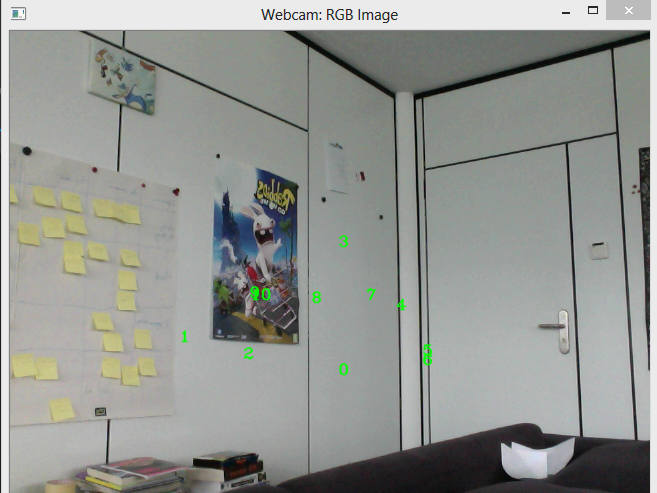
\includegraphics[scale=0.8]{images/calibration_points.png}
 	\captionof{figure}{Calibration points}
\end{center}

\begin{center}
	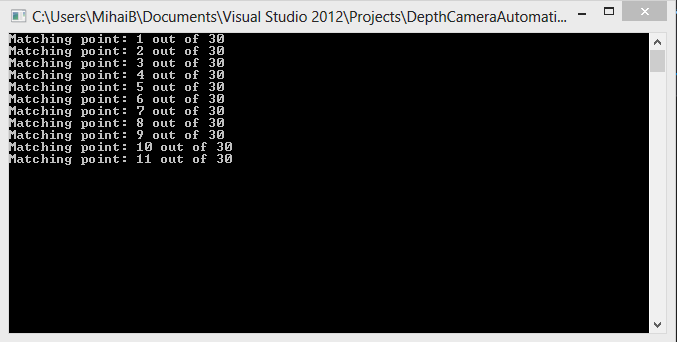
\includegraphics[scale=0.7]{images/console.png}
 	\captionof{figure}{Calibration console}
\end{center}

\begin{center}
	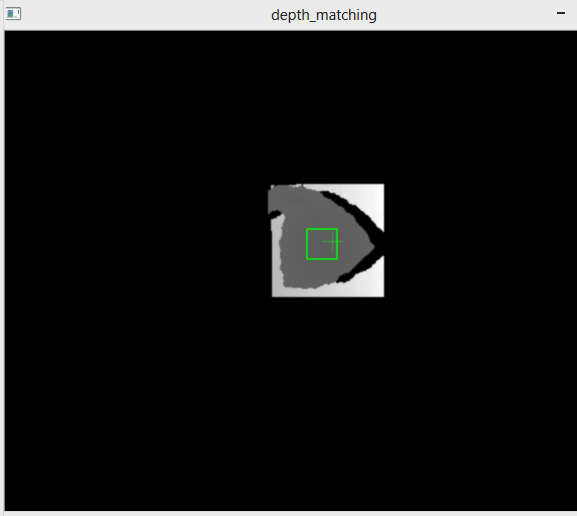
\includegraphics[scale=0.7]{images/good_kinect_depth_matching.png}
 	\captionof{figure}{Valid Kinect depth matching}
\end{center}

\begin{center}
	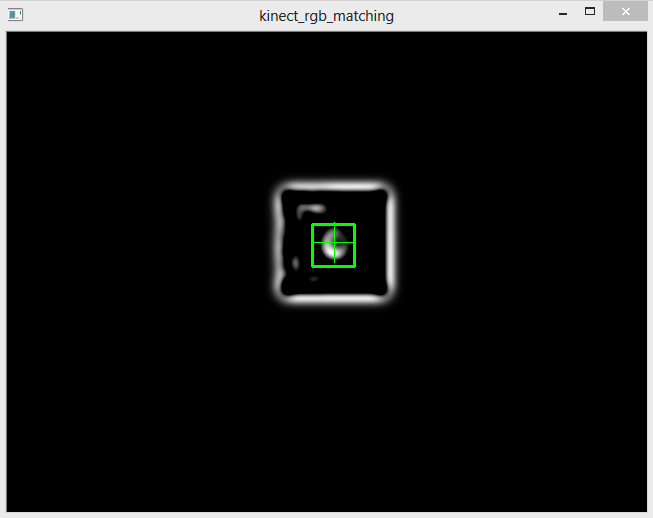
\includegraphics[scale=0.7]{images/good_kinect_rgb_matching.png}
 	\captionof{figure}{Valid Kinect RGB matching}
\end{center}

\begin{center}
	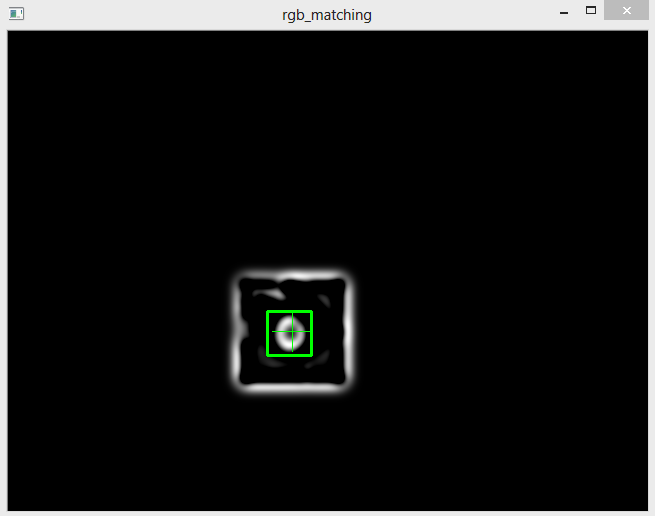
\includegraphics[scale=0.7]{images/good_rgb_matching.png}
 	\captionof{figure}{Valid webcam RGB matching}
\end{center}

\noindent
Once the calibration has been done, two new windows will appear. These windows represent the depth color reconstruction of the depth map based on the RGB image from the webcam. One window displays the image in 2D, while the other one displays the Kinect 3D point cloud. 

\begin{center}
	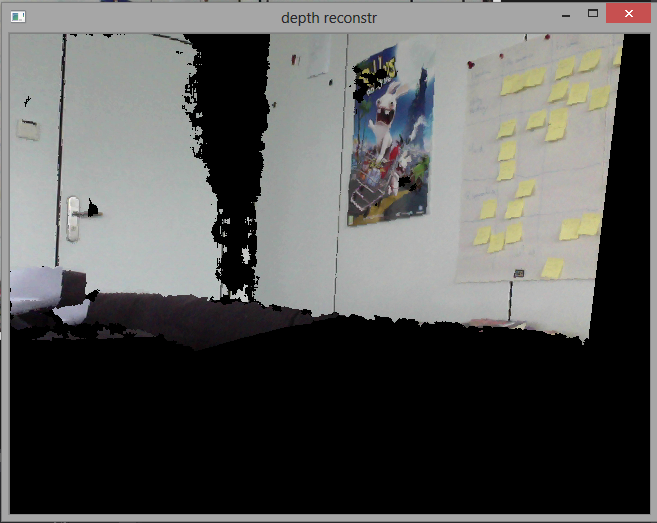
\includegraphics[scale=0.7]{images/depth_reconstruction_1.png}
 	\captionof{figure}{Depth color reconstruction}
\end{center}

\begin{center}
	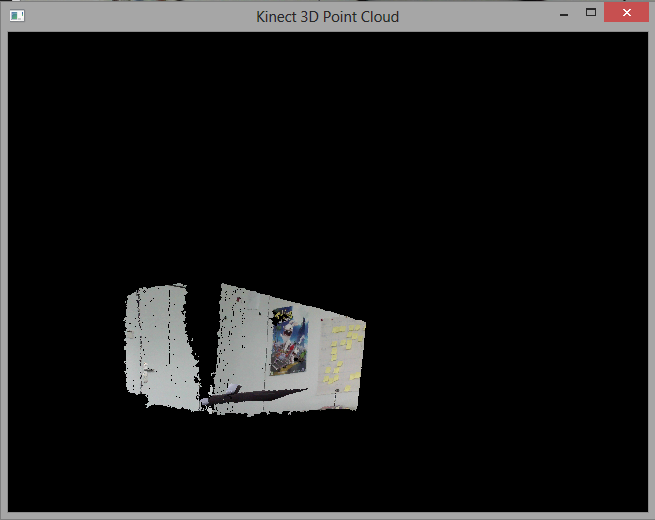
\includegraphics[scale=0.7]{images/point_cloud_1.png}
 	\captionof{figure}{Kinect 3D point cloud}
\end{center}

\begin{center}
	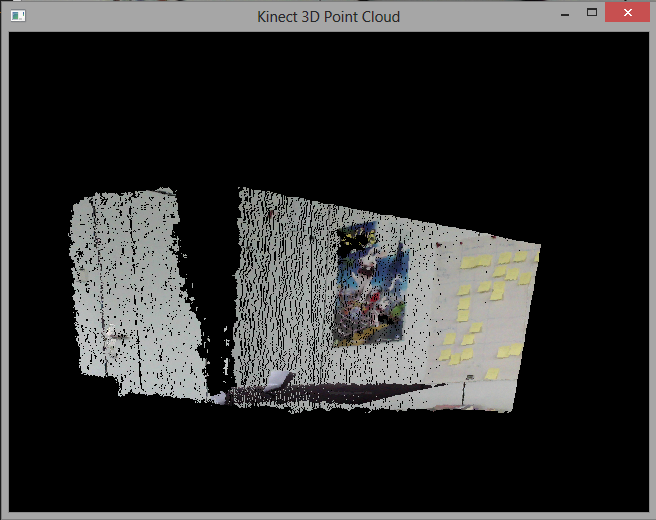
\includegraphics[scale=0.7]{images/point_cloud_2.png}
 	\captionof{figure}{Kinect 3D point cloud}
\end{center}

\begin{center}
	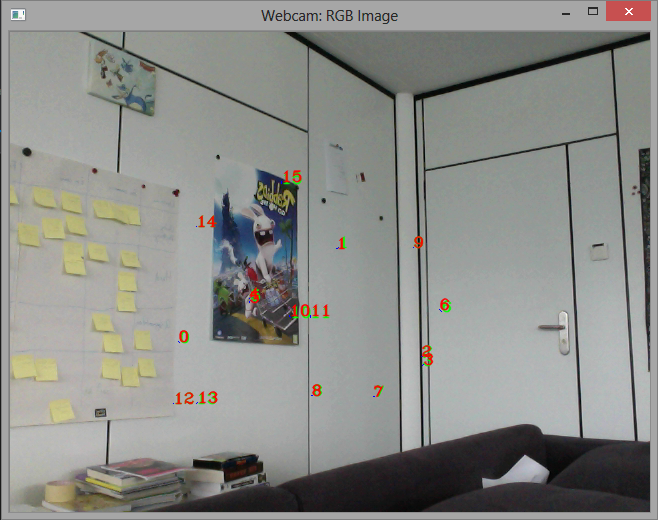
\includegraphics[scale=0.7]{images/depth_reconstruction_2.png}
 	\captionof{figure}{Reprojection of the collected points}
\end{center}

\noindent
We can also notice that the "Webcam: RGB Image" has changed. We will no longer have all the initial points, but only the points that have been kept after the iterative calibration process. We can also see the reprojections. A good calibration means that the reprojection is almost perfect, so there is no difference between the actual point detected and the point reprojected using the calibration. 

\subsection{3D point cloud scene control}
\noindent
The 3D point cloud is not just an image that one can look at. It is an environment where the user can navigate using some commands. The commands to controls the scene are described below.

\begin{itemize}
	\item w : Move in the $Z$ direction forward.
	\item a : Move in the $Z$ direction backwards.
	\item s : Strafe left ($X$ direction).
	\item d : Strafe right ($X$ direction).
	\item q : Move in the $Y$ direction up.
	\item e : Move in the $Y$ direction down.
	\item UP : Look up.
	\item DOWN : Look down.
	\item LEFT : Look left.
	\item RIGHT : Look right. 
\end{itemize}

\noindent
The controls have been made similarly to the ones found in a First Person Shooter (FPS) game. 
\\\\
\emph{Note:} For the controls to be active, the user must select the 3D point cloud window.

\section{Results}
\noindent
This section will describe the results of performing several calibrations and a comparison to the Kinect's calibration. Since we cannot test the calibration of the webcam with the calibration of the Kinect, we have performed another calibration for the Kinect. This way, we can test our calibration with the Kinect's default calibration. 

\subsection{Webcam calibration}
The minimum number of points required for a calibration is 6. However, we have seen in practice that 6 points are not enough for a good calibration. Taking into consideration that we do iterative improvement of the calibration, we need many more points since some of them will be eliminated (they are classified as outliers). One possible cause for correspondences to be considered outliers is due to the fact that the time difference between the RGB camera frame and the depth camera frame is not 0. If the pattern is quickly moving in the environment, the reprojection error might grow.  
\\\\
In practice, we have performed calibrations starting with 30 points. Once 30 points have been collected, the iterative calibration process begins. The table below shows the results that we have obtained with our calibration. 

\begin{center}
  \begin{tabular}{| c | c | c |}
    \hline
    Initial number of points & Final number of points & Calibration error \\ \hline
    30 & 18 & 2.3 \\ \hline
    30 & 12 & 2.1 \\ \hline
    30 & 8 & 2.8 \\
    \hline
  \end{tabular}
\end{center}

\noindent
The error is measured in pixels. An example of the result of the iterative calibration process can be seen below.

\begin{center}
	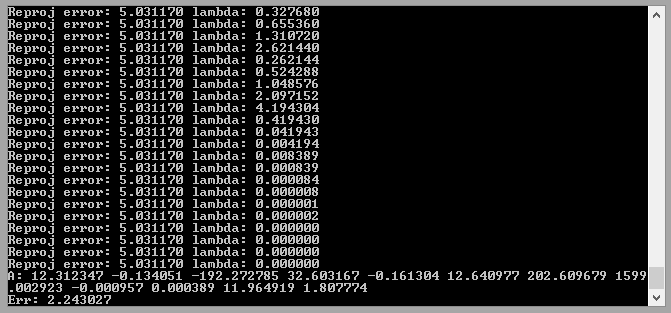
\includegraphics[scale=1]{images/webcam_calibration.png}
 	\captionof{figure}{Reprojection of the collected points}
\end{center}

\subsection{Comparison the the Kinect calibration}
\noindent
In order to compare our approach with the Kinect default calibration, we had to calibrate the Kinect. Once the Kinect has been calibrated we can compare the results of the two calibrations.
\\\\
How do we compare them?
\\\\
We take all the 3D points that have been kept in the calibrator and we reproject them on the Kinect's RGB Image. As reference points, we will consider the points that have been detected using the template matching process on the Kinect's RGB image. 

\begin{itemize}
	\item Let P3D(x,y,z) be a 3D point.
	\item We reproject P3D using our calibration and the reproject function described in the implementation. This will result in P\_ OUR(x,y).
	\item We reproject P3D using the Kinect's default calibration, using the function \emph{NuiImageGetColorPixelCoordinatesFromDepthPixelAtResolution}. We will get P\_ Kinect(x,y).
	\item We take as reference P\_ Ref(x,y) the point from the Kinect's RGB image, found using template matching.
\end{itemize}

\noindent
The goal is to be able to see which point, P\_ OUR or P\_ Kinect is closer to P\_ Ref. We have developed a visual and mathematical way to check. Some of the results that we have obtained can be seen below. 
\\\\
The mathematical way to verify the points is by computing the Euclidean distance between the target point (P\_ REF) and P\_ OUR and P\_ Kinect. The distance between them represents the error in pixels. The table below represents all the points that have been considered for a calibration, a total of 18 points. 

\begin{center}
  \begin{tabular}{| c | c | c |}
    \hline
    Id & Our Calibration Error & Kinect Calibration Error \\ \hline
    1 & 1 & 6.08276 \\ \hline
	2 & 1.41421 & 9 \\ \hline
	3 & 2 & 8.06226 \\ \hline
	4 & 1 & 8.06226 \\ \hline
	5 & 1 & 2 \\ \hline
	6 & 1 & 1.41421 \\ \hline
	7 & 1 & 2.23607 \\ \hline
	8 & 0 & 5 \\ \hline
	9 & 2.23607 & 5.38516 \\ \hline
	10 & 1 & 3 \\ \hline
	11 & 2 & 3.60555 \\ \hline
	12 & 2 & 2.82843 \\ \hline
	13 & 1 & 8.544 \\ \hline
	14 & 1.41421 & 9.05539 \\ \hline
	15 & 2 & 9.48683 \\ \hline
	16 & 1 & 7.07107 \\ \hline
  \end{tabular}
\end{center}

\begin{center}
	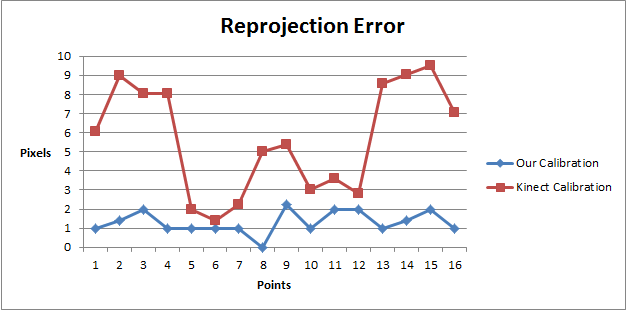
\includegraphics[scale=1]{images/chart.png}
 	\captionof{figure}{Visualization of the reprojection error}
\end{center}

\noindent
Below, you will see a series of pictures, where the points are presented in the context in which they were collected. In order to understand the comparison, each point is marked with a different color. 

\begin{itemize}
	\item \textcolor{blue}{BLUE} - The point which was detected with template matching.
	\item \textcolor{green}{GREEN} - The reprojection of the point found in the depth image using the calibration that we have developed.
	\item \textcolor{red}{RED} - The reprojection of the point found in the depth image using the calibration of the Kinect (the default calibration). 
\end{itemize}

\begin{center}
	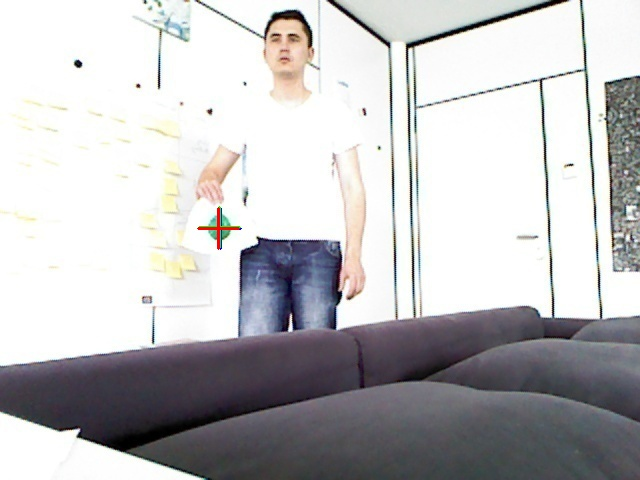
\includegraphics[scale=0.6]{images/compare_output/rgb_image_1.jpg}
 	\captionof{figure}{Reprojection of the collected points}
\end{center}

\begin{center}
	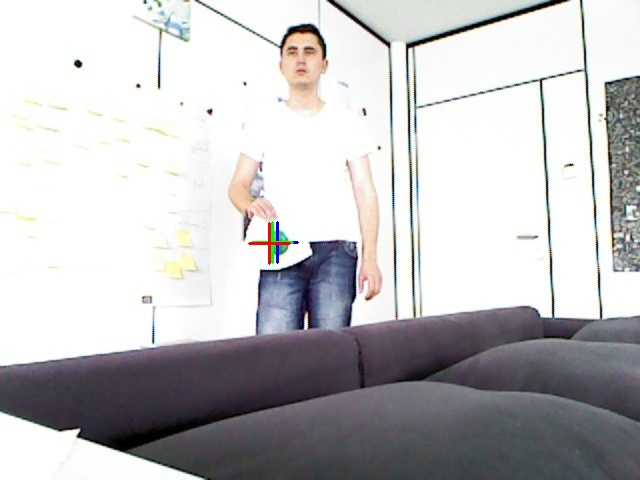
\includegraphics[scale=0.6]{images/compare_output/rgb_image_2.jpg}
 	\captionof{figure}{Reprojection of the collected points}
\end{center}

\begin{center}
	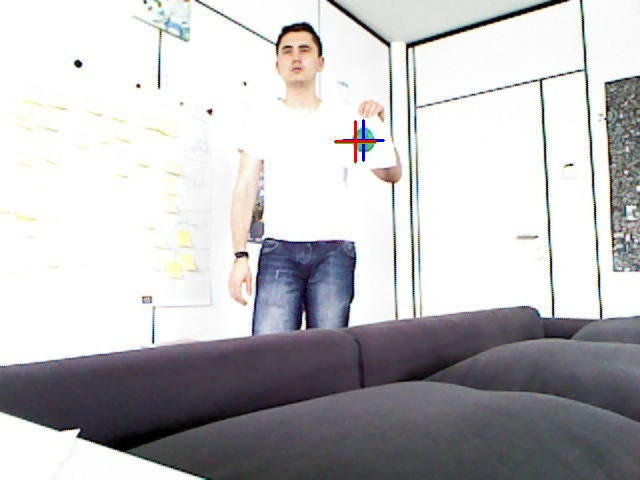
\includegraphics[scale=0.6]{images/compare_output/rgb_image_3.jpg}
 	\captionof{figure}{Reprojection of the collected points}
\end{center}

\begin{center}
	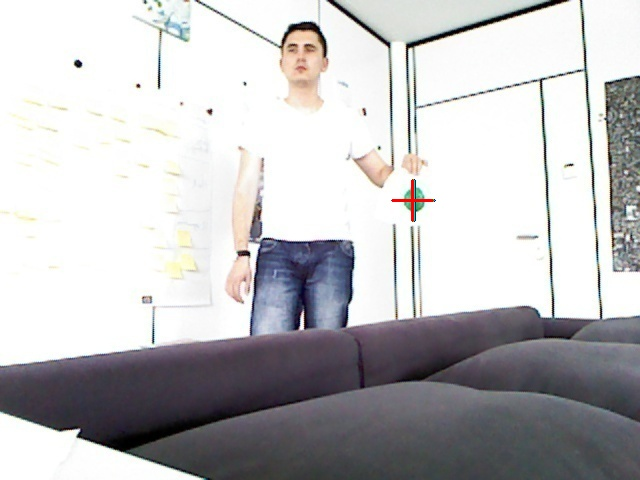
\includegraphics[scale=0.6]{images/compare_output/rgb_image_4.jpg}
 	\captionof{figure}{Reprojection of the collected points}
\end{center}

\begin{center}
	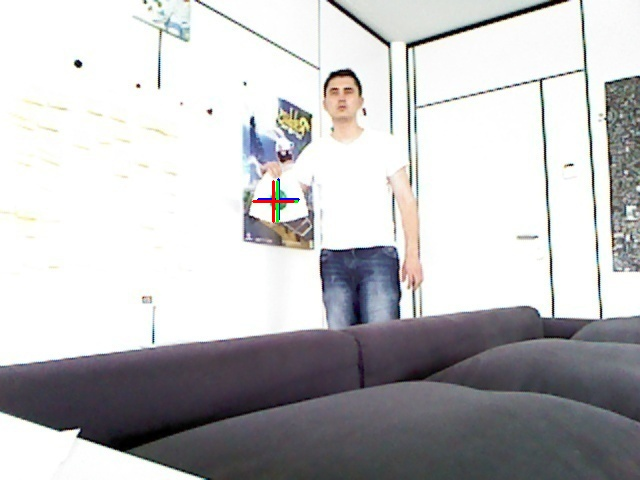
\includegraphics[scale=0.6]{images/compare_output/rgb_image_10.jpg}
 	\captionof{figure}{Reprojection of the collected points}
\end{center}

\begin{center}
	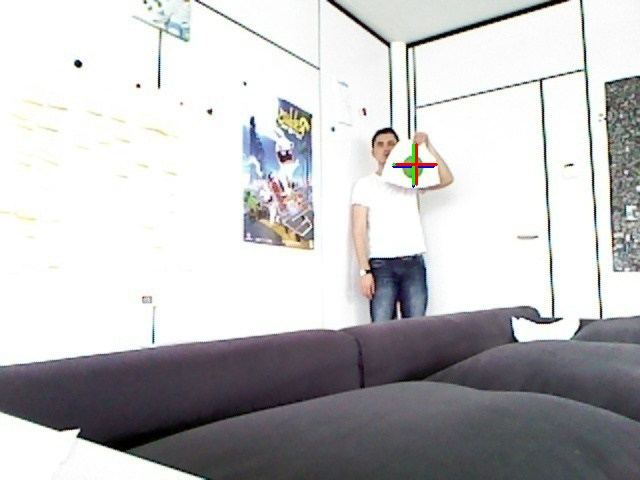
\includegraphics[scale=0.6]{images/compare_output/rgb_image_20.jpg}
 	\captionof{figure}{Reprojection of the collected points}
\end{center}

\begin{center}
	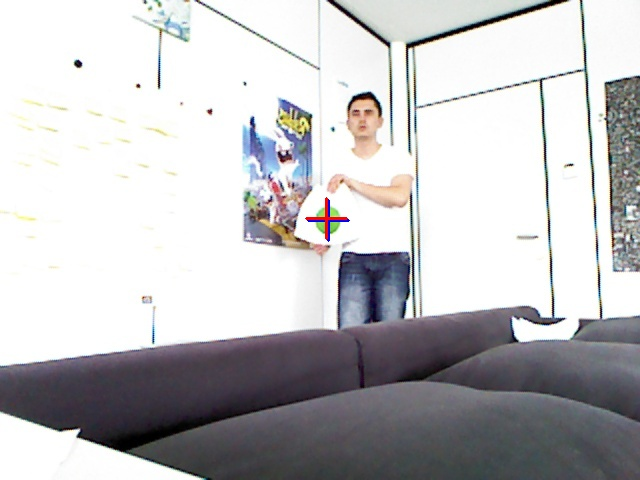
\includegraphics[scale=0.6]{images/compare_output/rgb_image_24.jpg}
 	\captionof{figure}{Reprojection of the collected points}
\end{center}